\let\counterwithout\relax
\let\counterwithin\relax
\documentclass[final]{fhnwreport}       %[mode] = draft or final
\usepackage{color, colortbl}
\usepackage{rotating, rotfloat,ragged2e, hyphenat}

                                        %{class} = fhnwreport, article, 
                                        %          report, book, beamer, standalone
%%---Main Packages-----------------------------------------------------------------------
\usepackage[english, ngerman]{babel}	%Mul­tilin­gual sup­port for LaTeX
\usepackage[T1]{fontenc}				%Stan­dard pack­age for se­lect­ing font en­cod­ings
\usepackage[utf8]{inputenc}				%Ac­cept dif­fer­ent in­put en­cod­ings
\usepackage{lmodern}                    %The newer Font-Set
\usepackage{textcomp}					%LaTeX sup­port for the Text Com­pan­ion fonts
\usepackage{graphicx} 					%En­hanced sup­port for graph­ics
\usepackage{float}						%Im­proved in­ter­face for float­ing ob­jects
\usepackage{ifdraft}                    %Let you check if the doc is in draft mode

%%---Useful Packages---------------------------------------------------------------------
\usepackage[pdftex,dvipsnames]{xcolor}  %Driver-in­de­pen­dent color ex­ten­sions for LaTeX
\usepackage{csquotes}                   %Simpler quoting with \enquote{}
\usepackage{siunitx} 					%A com­pre­hen­sive (SI) units pack­age
\usepackage{listings}					%Type­set source code list­ings us­ing LaTeX
\usepackage[bottom]{footmisc}			%A range of foot­note op­tions
\usepackage{footnote}					%Im­prove on LaTeX's foot­note han­dling
\usepackage{verbatim}					%Reim­ple­men­ta­tion of and ex­ten­sions to LaTeX ver­ba­tim
\usepackage[textsize=footnotesize]{todonotes} %Mark­ing things to do in a LaTeX doc­u­ment

%%---Tikz Packages-----------------------------------------------------------------------
\usepackage{standalone}
\usepackage{tikz}
\usepackage{circuitikz}
\usetikzlibrary{arrows}
\usetikzlibrary{calc}
\usetikzlibrary{intersections}

%%---Math Packages-----------------------------------------------------------------------
\usepackage{amsmath}					%AMS math­e­mat­i­cal fa­cil­i­ties for LaTeX
%\usepackage{amssymb}					%Type­set­ting symbols (AMS style)
%\usepackage{array}						%Ex­tend­ing the ar­ray and tab­u­lar en­vi­ron­ments
%\usepackage{amsthm}					%Type­set­ting the­o­rems (AMS style)

%%---Table Packages----------------------------------------------------------------------
\usepackage{tabularx}					%Tab­u­lars with ad­justable-width columns
%\usepackage{longtable}
\usepackage{multirow}					%Create tab­u­lar cells span­ning mul­ti­ple rows
\usepackage{multicol}					%In­ter­mix sin­gle and mul­ti­ple columns

%%---PDF / Figure Packages---------------------------------------------------------------
\usepackage{pdfpages}					%In­clude PDF doc­u­ments in LaTeX
\usepackage{pdflscape}					%Make land­scape pages dis­play as land­scape
\usepackage{subfig}					    %Fig­ures di­vided into sub­fig­ures

%%---Other Packages----------------------------------------------------------------------
%\usepackage{xargs}                     %De­fine com­mands with many op­tional ar­gu­ments

%%---Bibliography------------------------------------------------------------------------
\usepackage[style=ieee,urldate=comp,backend=biber]{biblatex}
\addbibresource{literature/bibliography.bib}

%%---Main Settings-----------------------------------------------------------------------
\graphicspath{{./graphics/}}			%Defines the graphicspath
%\geometry{twoside=false}				    %twoside=false disables the "bookstyle"
\setlength{\marginparwidth}{2cm}
\overfullrule=5em						%Creates a black rule if text goes over the margins => debugging


%%---User Definitions--------------------------------------------------------------------
%%Tabel-Definitions: (requires \usepackage{tabularx})
\newcolumntype{L}[1]{>{\raggedright\arraybackslash}p{#1}}    %column-width and alignment
\newcolumntype{C}[1]{>{\centering\arraybackslash}p{#1}}
\newcolumntype{R}[1]{>{\raggedleft\arraybackslash}p{#1}}

%%---Optional Package Settings-----------------------------------------------------------
%Listings-Settings: (requires \usepackage{listings}) => Example with Matlab Code
\lstset{language=Matlab,%
    basicstyle=\footnotesize\ttfamily,
    breaklines=false,%
    morekeywords={switch, case, otherwise},
    keywordstyle=\color{Blue},%
    tabsize=2,
    %morekeywords=[2]{1}, keywordstyle=[2]{\color{black}},
    identifierstyle=\color{Black},%
    stringstyle=\color{Purple},
    commentstyle=\color{Green},%
    showstringspaces=false,%without this there will be a symbol in the places where there is a space
    numbers=left,%
    numberstyle={\tiny \color{black}},% size of the numbers
    numbersep=9pt, % this defines how far the numbers are from the text
    %emph=[1]{word1, word2,...},emphstyle=[1]\color{red}
}							
			                %loads all packages, definitions and settings												
\title{«DJ» EMI Filter für Schaltnetzteil}          			%Project Title
\author{Pflichtenheft organisatorischer Teil}   %Document Type => Technical Report, ...
\date{Windisch, 23.03.2019}             		%Place and Date

\begin{document}

%%---TITLEPAGE---------------------------------------------------------------------------
\selectlanguage{ngerman}                %ngerman or english
\maketitle

\vspace*{-1cm}						    %compensates the space after the date line.
\vfill
\begin{figure}[H]
\centering
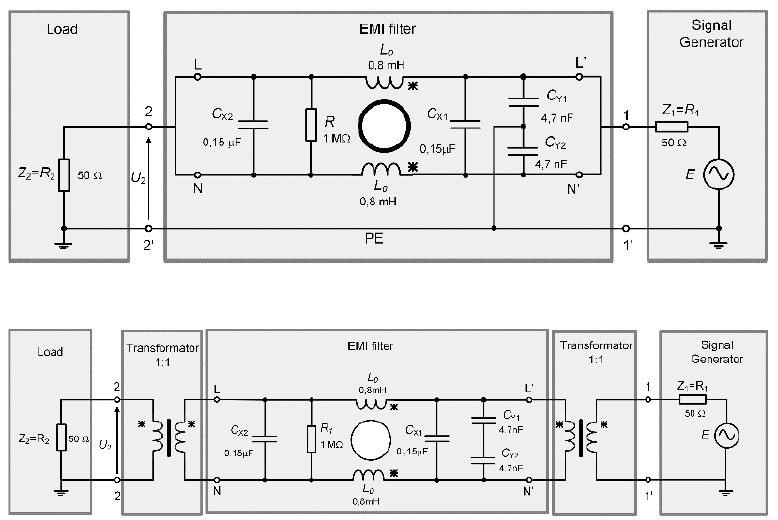
\includegraphics[width=10cm]{titelBild.png}
\end{figure}
\vfill

{
\renewcommand\arraystretch{2}
\begin{center}
\begin{tabular}{ >{\bf} l p{10cm} l }
Hochschule&Hochschule für Technik - FHNW\\
Studiengang&Elektro- und Informationstechnik\\
Auftraggeber&Dr. Luca Dalessandro\\
Betreuer&Prof. Dr. Sebastian Gaulocher \newline Prof. Peter Niklaus \newline Prof. Dr. Richard Gut \newline  Dr. Anita Gertiser \newline Pascal Buchschacher \\
Autoren&\textbf{Gruppe 1} \newline Niklaus Schwegler \newline Marco Binder \newline Lukas von Däniken \newline Pascal Puschmann \newline Claudio Alfare \newline Simon Rohrer \\
Version&1.0 %Normally not used!
\end{tabular}
\end{center}
}

\clearpage

%\selectlanguage{ngerman}				%ngerman or english
\thispagestyle{empty}
			
%%---TABLE OF CONTENTS-------------------------------------------------------------------
\pagenumbering{Roman}		
%\selectlanguage{ngerman}				%ngerman or english
\tableofcontents
\clearpage

%%---TEXT--------------------------------------------------------------------------------
\pagenumbering{arabic}
\section{Einleitung} \label{sec:einleitung}
Entwurf Einleitung P2 EMI-Filter Team 1

Gemäss des Lastenhefts wurde der Auftrag erteilt, eine Simulationssoftware zu entwickeln. Diese Simulationssoftware soll die Einfügedämpfung eines EMI-Filters simulieren und grafisch darstellen. EMI-Filter werden üblicherweise in Schaltnetzteile verbaut, um zu verhindern, dass Störungen zurück ins Netz gespeist werden. Netzgeräte können unter Umständen hohe Frequenzen erzeugen, die sich nicht gut mit der Netzfrequenz von 50 Hz vertragen. Der EMI-Filter filtert genau diese hochfrequenten Signale heraus, um zu verhindern, dass andere Geräte, die auch ans Netz angeschlossen werden, nicht davon beeinträchtigt werden.

Um die Einfügedämpfung zu ermitteln, soll das EMI-Filter bezüglich der Gleich- und Gegentaktschaltung untersucht werden. Dies geschieht anhand zweier Funktionen für Gleich- und Gegentaktschaltung. Die Funktionen zeigen die Einfügdämpfung für einen Frequenzbereich bis 30MHz.Die beiden Schaltungen beinhalten die parasitären Parameter der elektrischen Komponenten, sodass eine möglichst wahrheitsgetreue Simulation gemacht werden kann. Die entwickelte Software soll die Einfügedämpfung grafisch darstellen.  Die Resultate werden für die Gleich- und Gegentaktschaltung in separaten Funktionen dargestellt. Des Weiteren sollen die elektrischen Komponenten der Schaltungen in der Simulationssoftware variiert werden können.
 
Damit sichergestellt werden kann, dass die Simulationen mathematisch korrekt sind, werden alle Berechnungen zuerst in MATLAB durchgerechnet. Diese Ergebnisse werden mit Simulationen der Simulationssoftware MPLAB MINDI verglichen. Des Weiteren wird überprüft, wie die Schaltung vereinfacht werden kann. Dies erfolgt einerseits durch Symmetrien der Schaltung, was dazu führt, dass Komponenten zusammengefasst werden können. Andererseits auch durch Weglassen aufgrund von vernachlässigbarem Einfluss auf die Simulationen. Die Softwarestruktur orientiert sich am gängigen Prinzip der MVC(Model-View-Control). Diese Strukturierung begünstigt einen modularen Aufbau, was die Software einfach erweiterbar macht und zudem eine unkomplizierte Wartung ermöglicht. Des Weiteren wird die Software anhand des Testkonzepts Modul für Modul getestet.

Im Fokus des Fachberichts befindet sich die Software, da das zu entwickelnde Produkt eine Simulationssoftware ist. Der Fachbericht ist nach dem Top-Down-Prinzip aufgebaut. In einem ersten Schritt wird die Software als Ganzes Beschrieben. In den darauffolgenden Kapiteln befinden sich die Dokumentationen der beiden Teile der Software. Die Software wird aufgegliedert in den Teil Benutzeroberfläche und den Teil Ermittlung der Einfügedämpfung. Um den Fachbericht schlank zu gestalten, werden sämtliche theoretische Grundlagen im Anhang platziert. Falls in Kapiteln entsprechende Theorie wichtig ist wird darauf verwiesen.


\section{Projektorganisation}

Die Studierenden werden im Projekt 1 (pro1E) für den Studiengang Elektro- und Informationstechnik von drei Dozenten der Fachhochschule Nordwestschweiz (FHNW) unterstützt. Pascal Buchschacher informiert über Projektmanagement allgemein, Anita Gertiser vermittelt den Studenten die richtige Kommunikation innerhalb des Teams und Felix Jenni steht als Ansprechpartner für Fragen technischer Natur zur Verfügung.
\subsection{Projektverantwortliche}

\subsection{Auftraggeber}
Auftraggeber des Projekts 1 ist Felix Jenni, Dozent an der Fachhochschule Nordwestschweiz.

\subsection{Teammitglieder}
Das Team 3 des Projekts 1 setzt sich aus sechs Studenten der Fachhochschule Nordwestschweiz, Hochschule für Technik in Brugg/Windisch zusammen. Frank Imhof (FI) ist der Projektleiter und verantwortlich für die Arbeiten und die Kommunikation mit dem Auftraggeber und den Fachdozenten. Unterstützt wird dieser vom stellvertretenden Projektleiter \newline Pascal Puschmann (PP). Die übrigen Mitglieder sind Michel Alt (MA), Lars Bachmann (LB), Roni Fischer(RB) und Christoph Kuhn(CK). Jeder von ihnen studiert Elektro- und Informationstechnik im ersten Semester, mit Ausnahme von Christoph Kuhn, der gleichzeitig das Projekt 3 absolviert.

\subsection{Organigramm}
\begin{figure}[H]
	\centering
	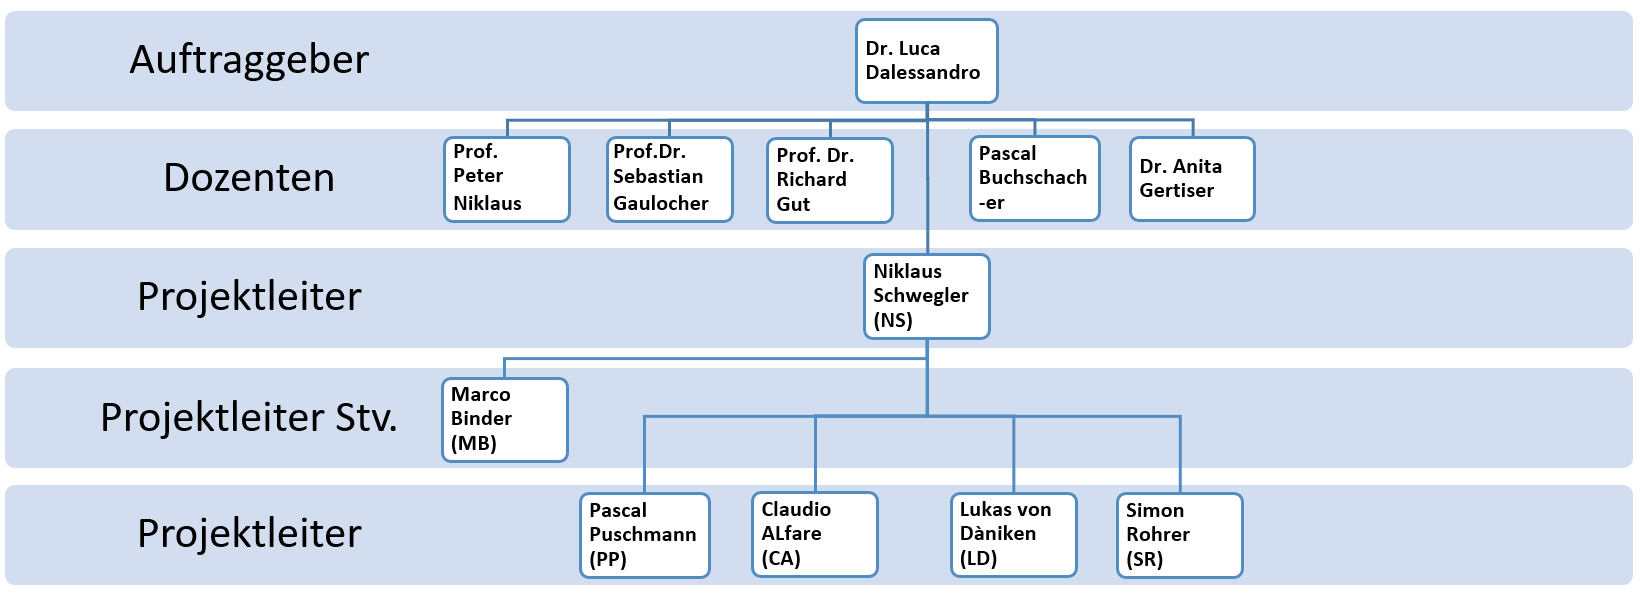
\includegraphics[width=10cm]{Organi.png}
	\label{fig:Organigramm}
\end{figure}

\section{Projektplan}

\subsection{Projektzeitplan/ Projektstrukturplan}
\begin{figure}[H]
	\centering
	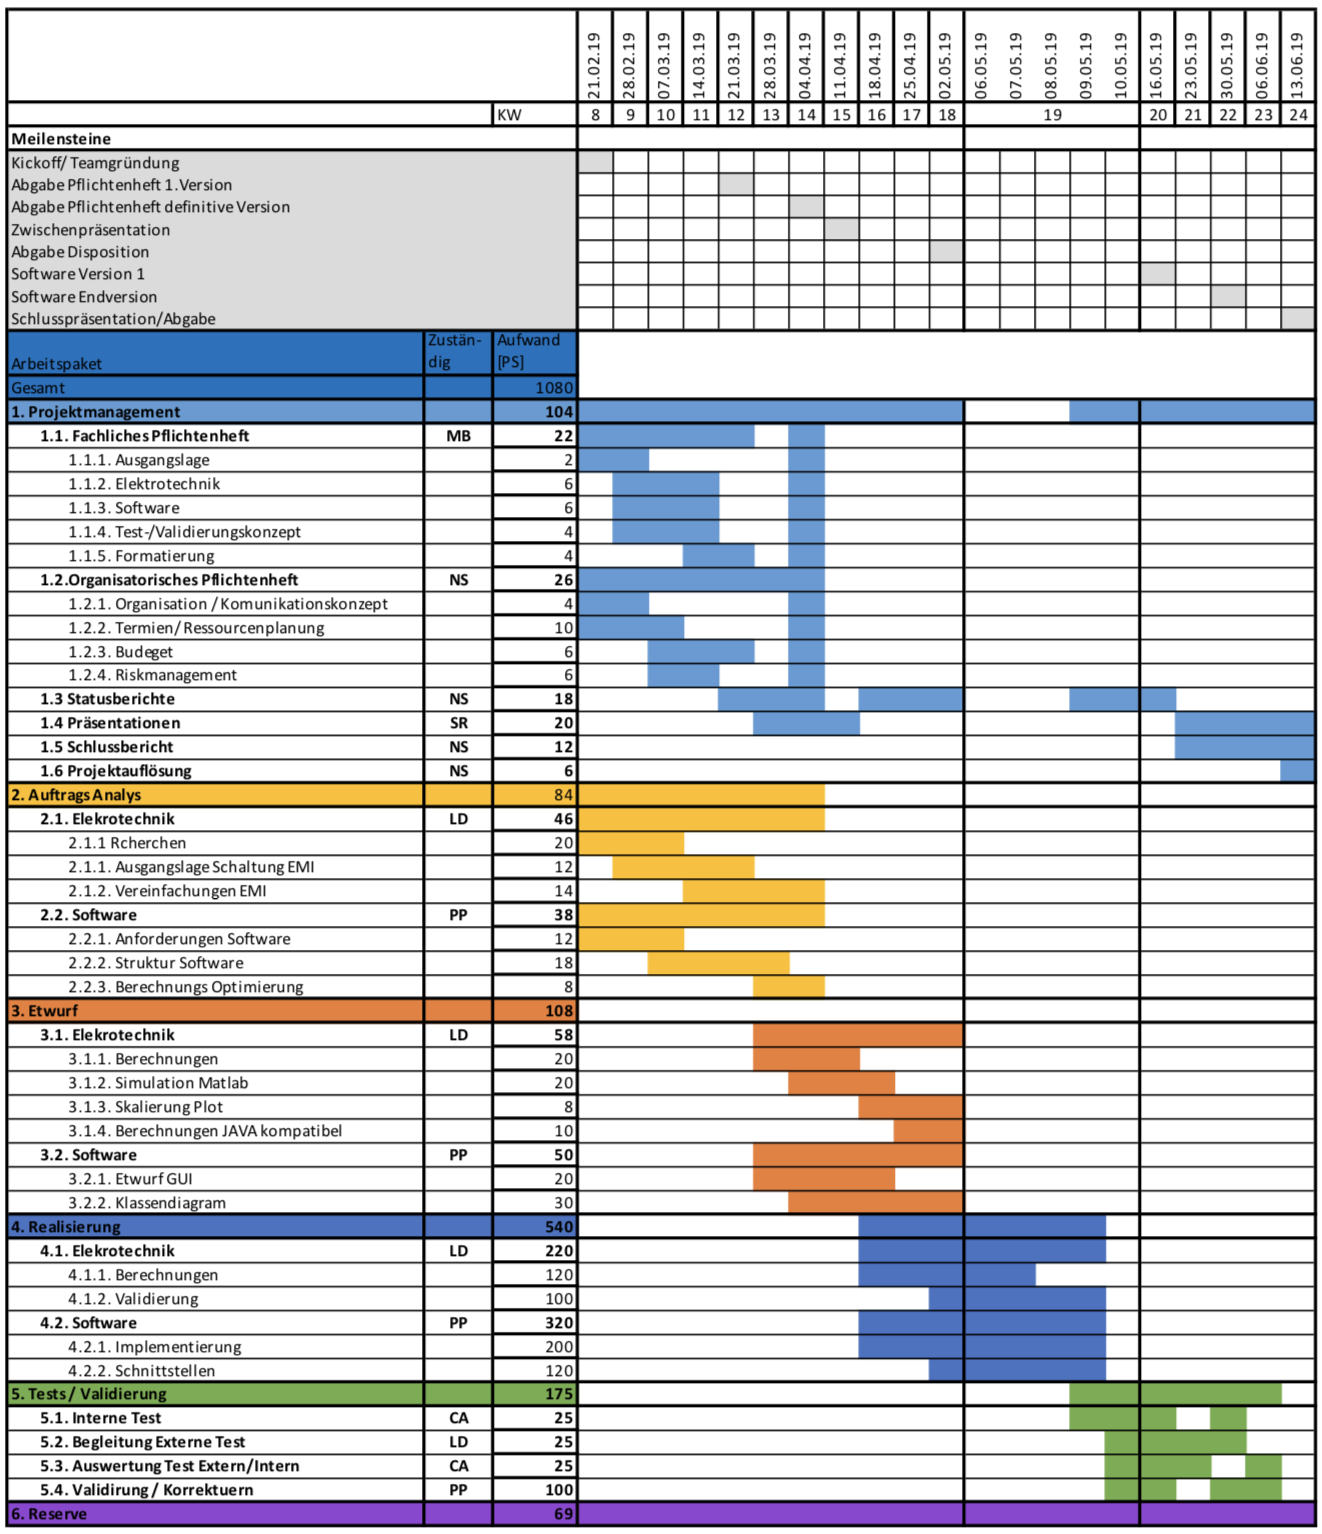
\includegraphics[width=16cm]{Terminplan_P2.png}
	\label{fig:Terminplan}
\end{figure}




\renewcommand{\arraystretch}{1.2}
\definecolor{grau}{gray}{0.9}
\definecolor{hellgrau}{gray}{0.95}
\section{Projektbudget}
%\subsection{Personalaufwand}
Für das Erstellen des Budgets wurden folgende Salär-Ansätze verwendet: 
\begin{table}[H]
\begin{tabular}{ll}
Projektleiter:      & 148 CHF/h (nur für Phase Projektmanagement) \\
Projektmitarbeiter: & 74 CHF/h                                   
\end{tabular}
\end{table}

%% Please add the following required packages to your document preamble:
% \usepackage[table,xcdraw]{xcolor}
% If you use beamer only pass "xcolor=table" option, i.e. \documentclass[xcolor=table]{beamer}
\begin{table}[H]
\small
\begin{tabular}{l|r|r|r|r}
\textbf{Phase}       & \textbf{Stunden} & \textbf{Stundenanteil} & \textbf{Kosten}         & \textbf{Kostenanteil}\\ \hline
1. Analyse           &193               & 39\%                 &  CHF 14'282.00           & 36\%   \\ \hline
2. Entwurf           &207               & 41\%                 &  CHF 15'318.00           & 39\%   \\ \hline
3. Projektmanagement &33               & 7\%                 &  CHF 4'884.00           &  12\%   \\ \hline
4. Dokumentation     &25               & 5\%                 &  CHF 1'850.00           & 5\%   \\ \hline
5. Reserve           & 40               & 8\%                 &  CHF 2'960.00           & 8\%   \\ \hline
\rowcolor{grau} 
\textbf{TOTAL}       & \textbf{498}     &\textbf{100\%}          &\textbf{CHF 39'294.00}   &\textbf{100\%}
\end{tabular}
\end{table}

\begin{table}[H]
\begin{tabular}{ll}
Gesamtkosten: 	 		& CHF 39'442.00 \\
Total Stunden:			& 498			\\	
Anzahl Teammitglieder:	& 5.5			\\
Stunden pro Person: 	& 90.5			                              
\end{tabular}
\end{table}
\section{Kommunikationskonzept}
\begin{figure}[H]
	\centering
	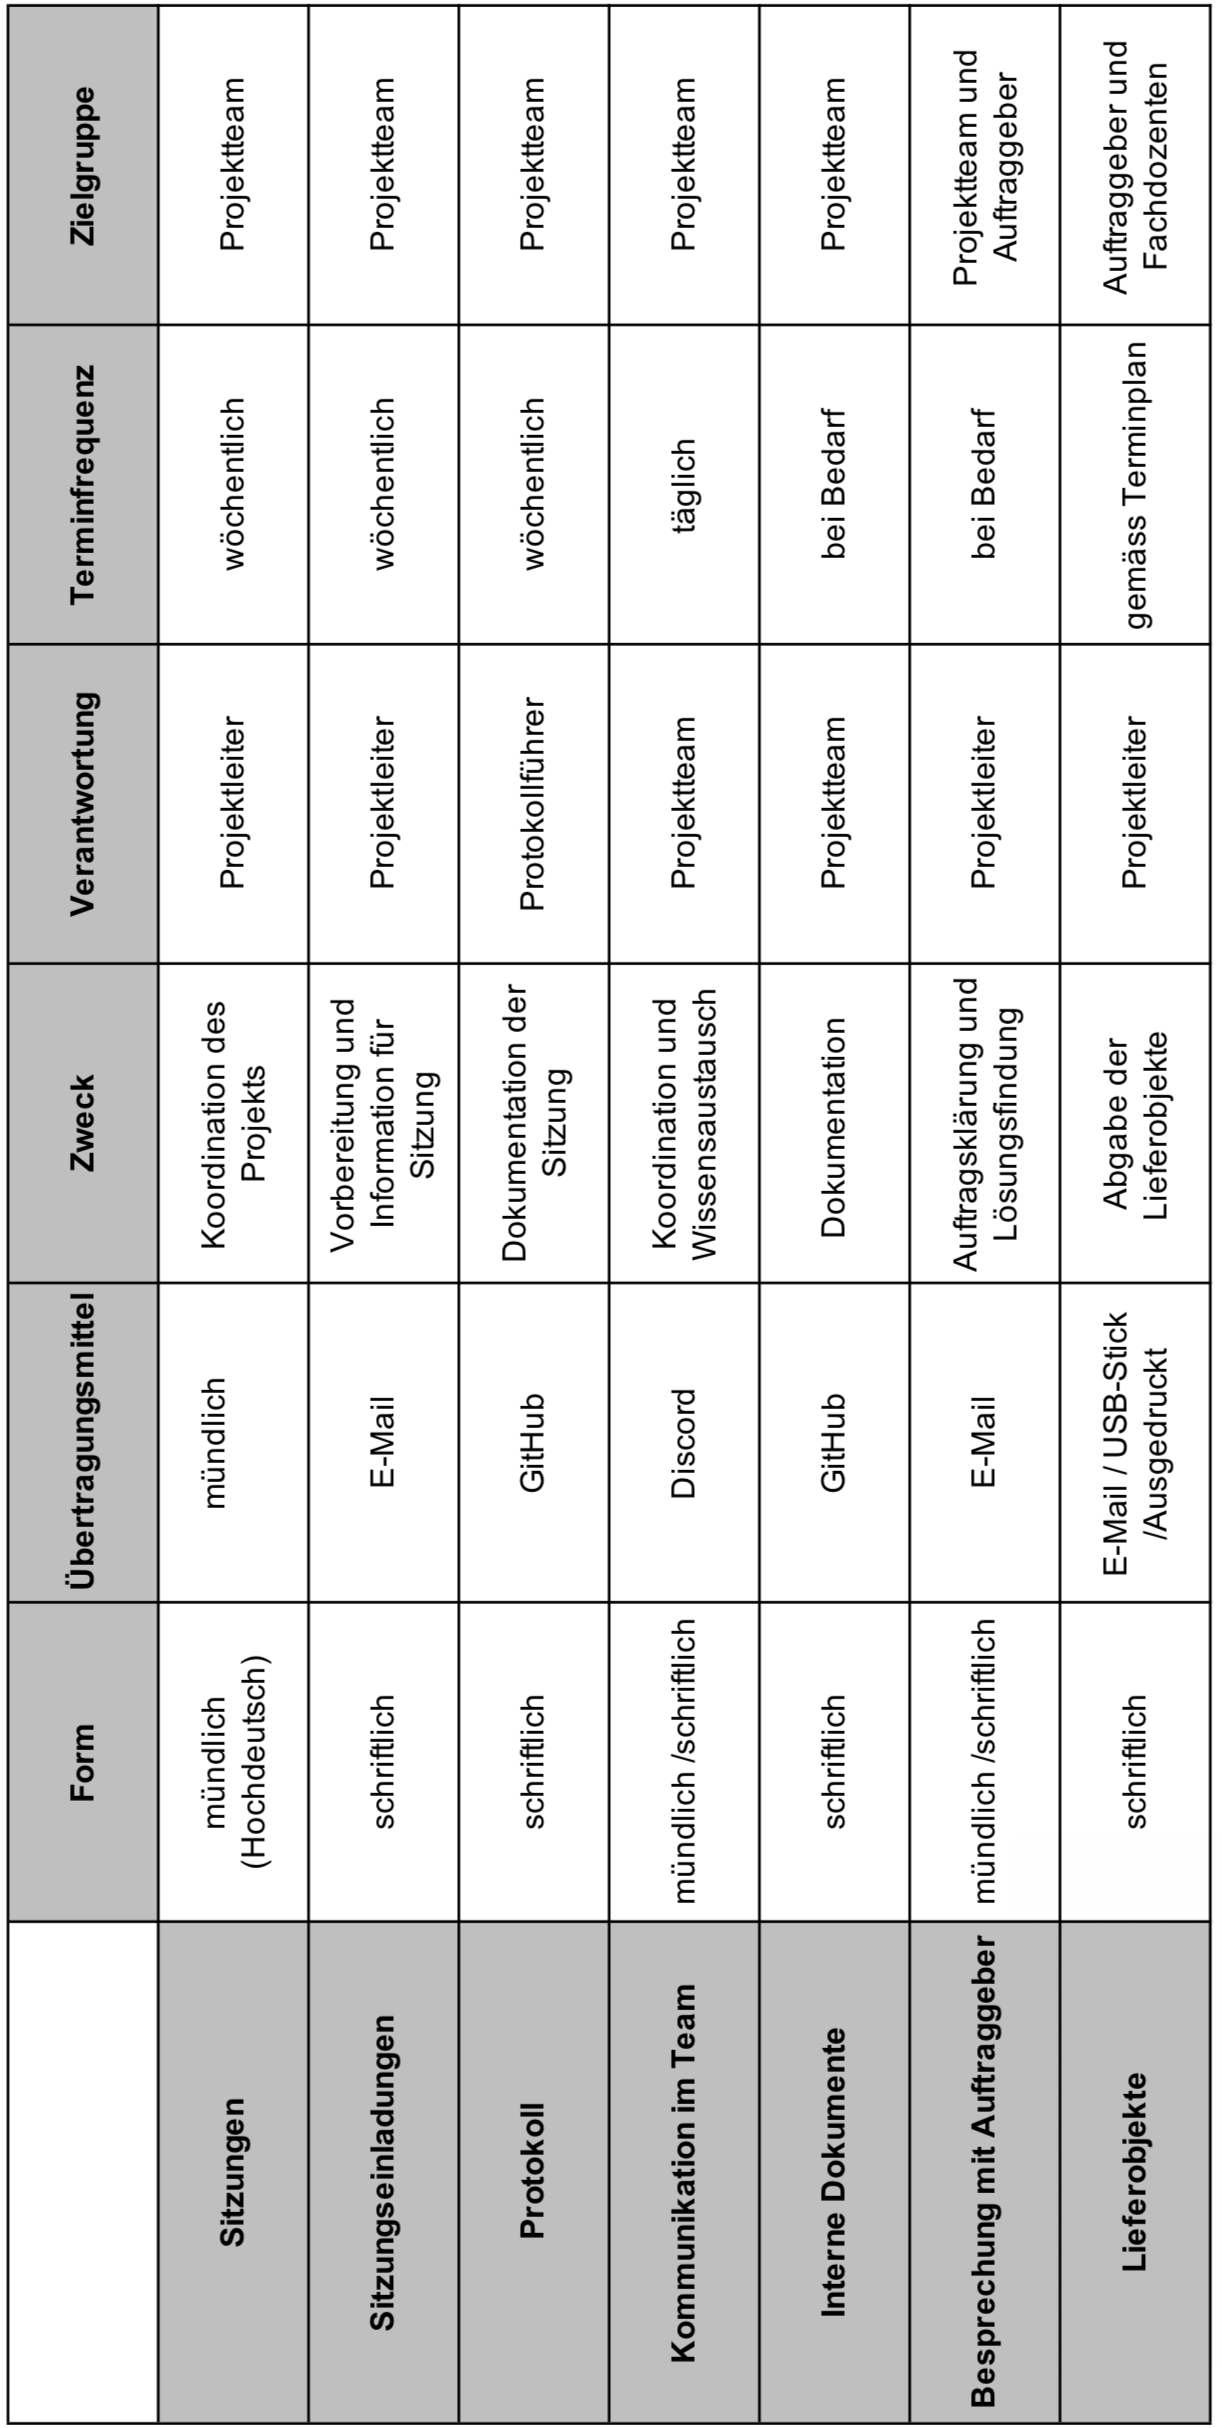
\includegraphics[width=10cm]{Kommunikationskonzept_P2.png}
	\label{fig:Kommunikationskonzept}
\end{figure}


\section{Risikoanalyse}

Risiken werden während der Projektplanung ebenfalls eruiert und tabellarischkategorisiert. Dabei werden ebenfalls Folgerisiken und Dringlichkeit beurteilt. Um diesen Risiken entgegenzuwirken werden Präventionsmassnahmen ausgearbeitet und implementiert. 
\\
\\
\\
\\
\\

\begin{figure}[H]
	\centering
	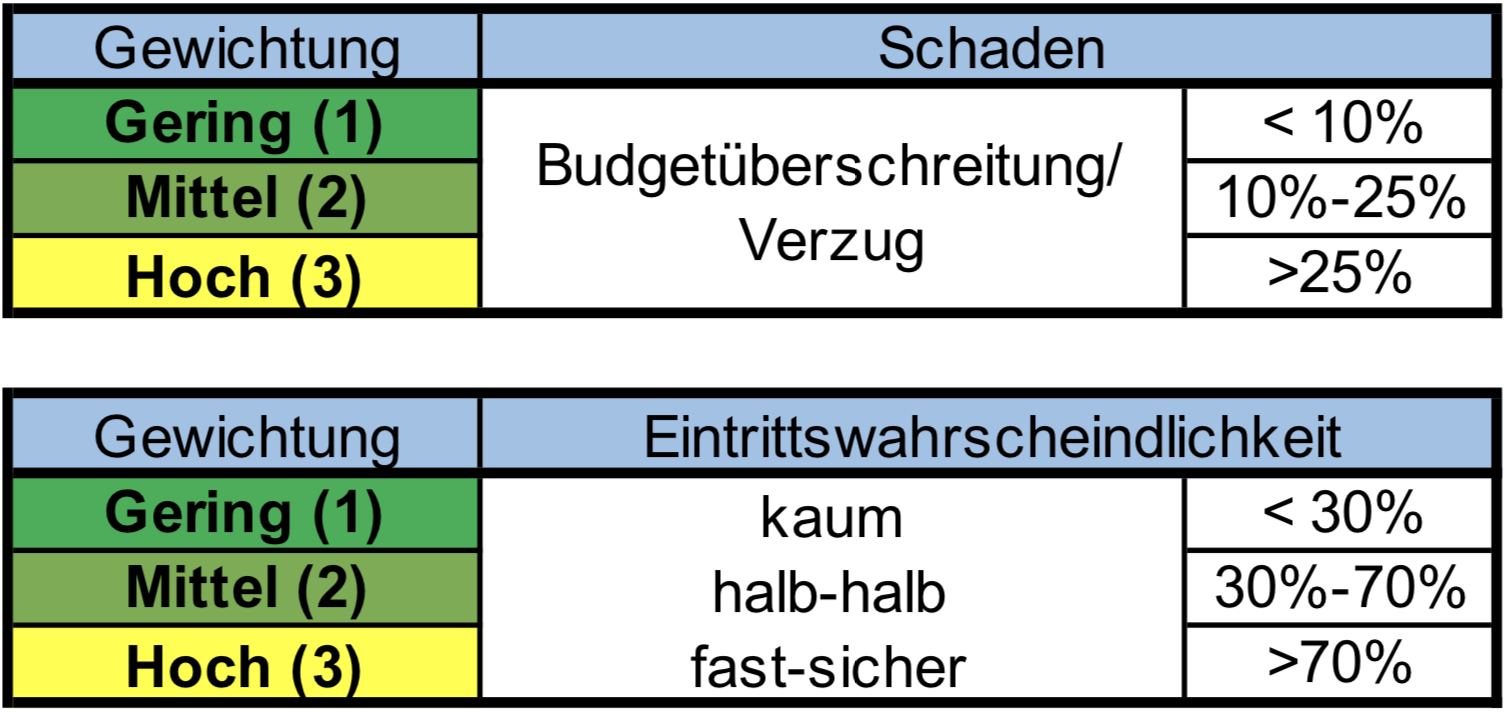
\includegraphics[width=14cm]{Gewichtung_P2.png}
	\label{fig:Gewichtung}
\end{figure}

\newpage



\begin{figure}[H]
\centering
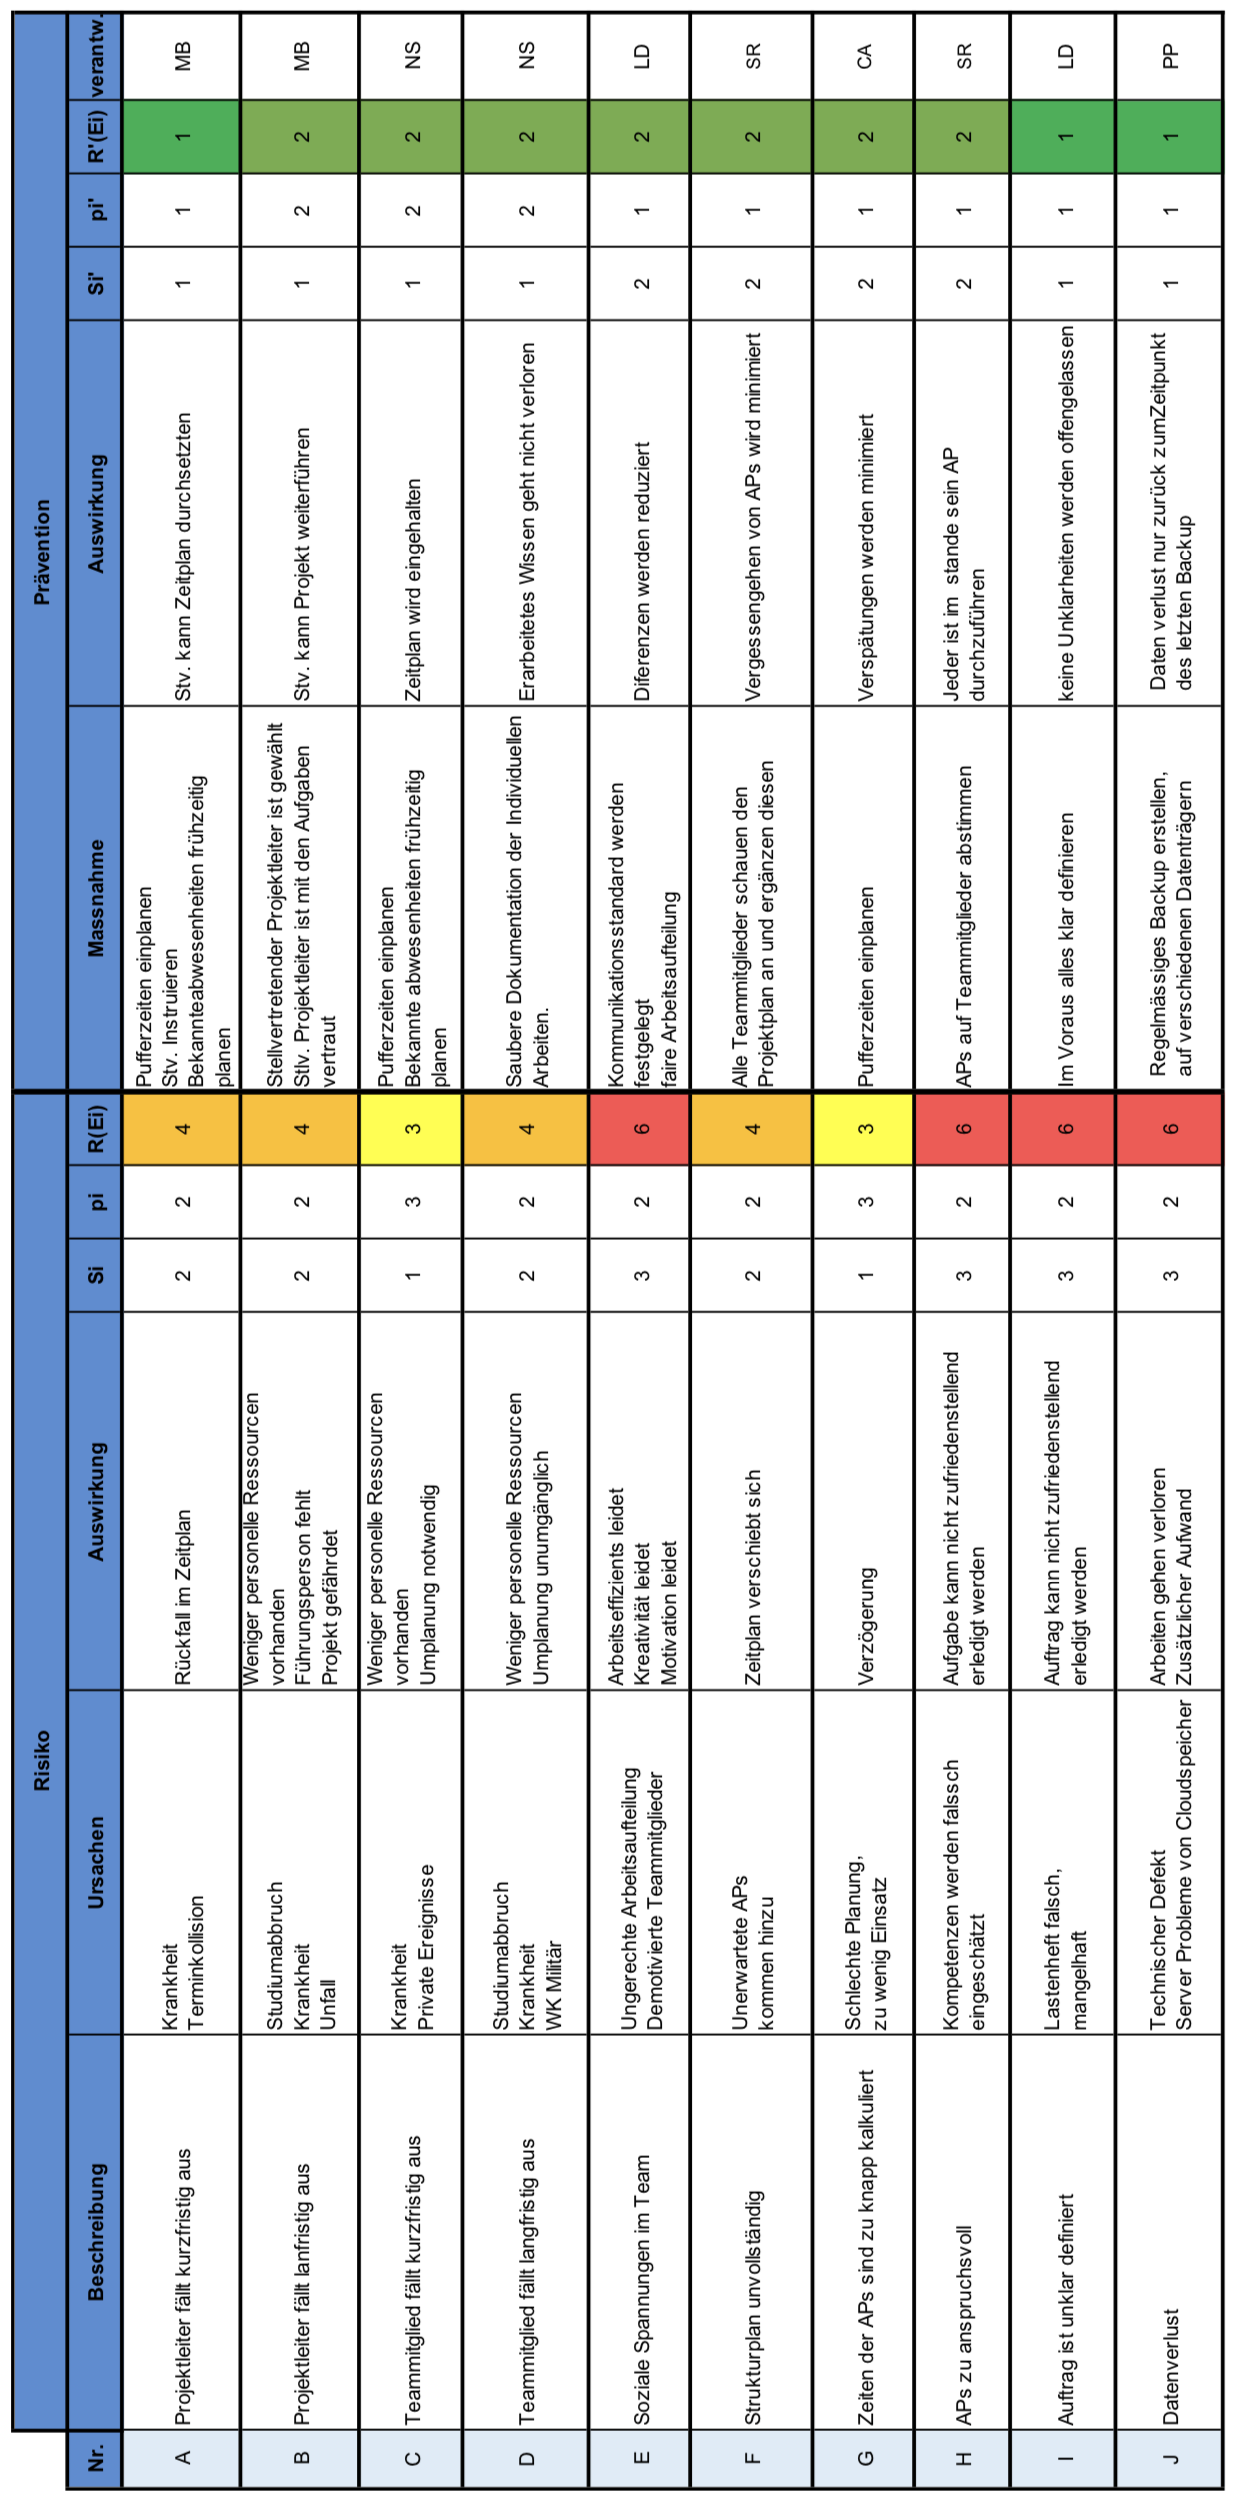
\includegraphics[width=12.5cm]{Risikotabelle_P2.png}
\label{fig:Risikotabell}
\end{figure}

\newpage
\begin{figure}[H]
	\centering
	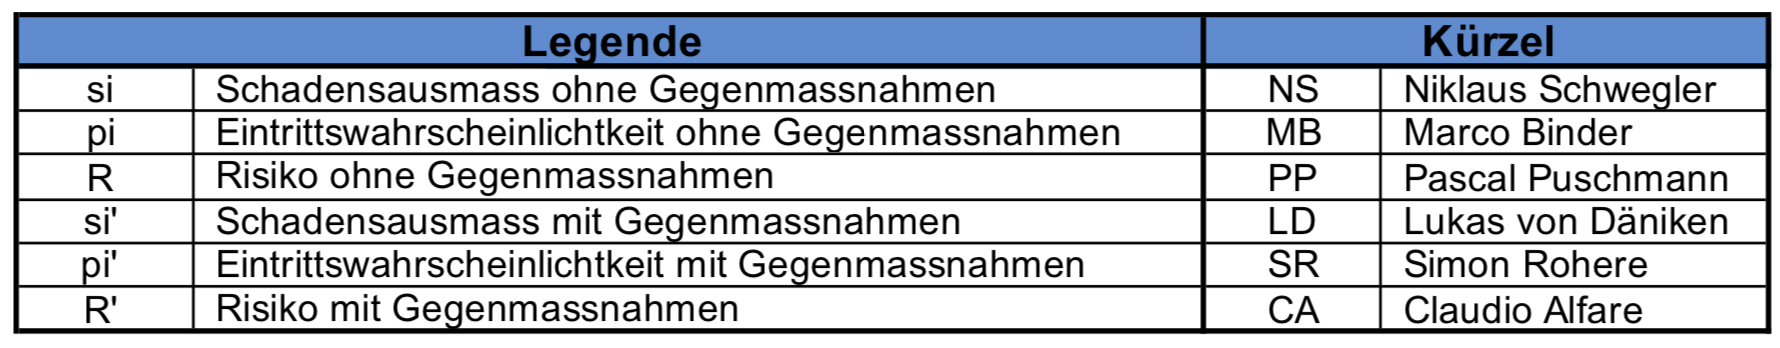
\includegraphics[width=14cm]{Legende_P2.png}
	\label{fig:Tabelle}
\end{figure}







Auf der folgenden Risikomap sind alle Gefahren jeweils mit und ohne Präventionsmassnahme graphisch dargestellt.

\begin{figure}[H]
	\centering
	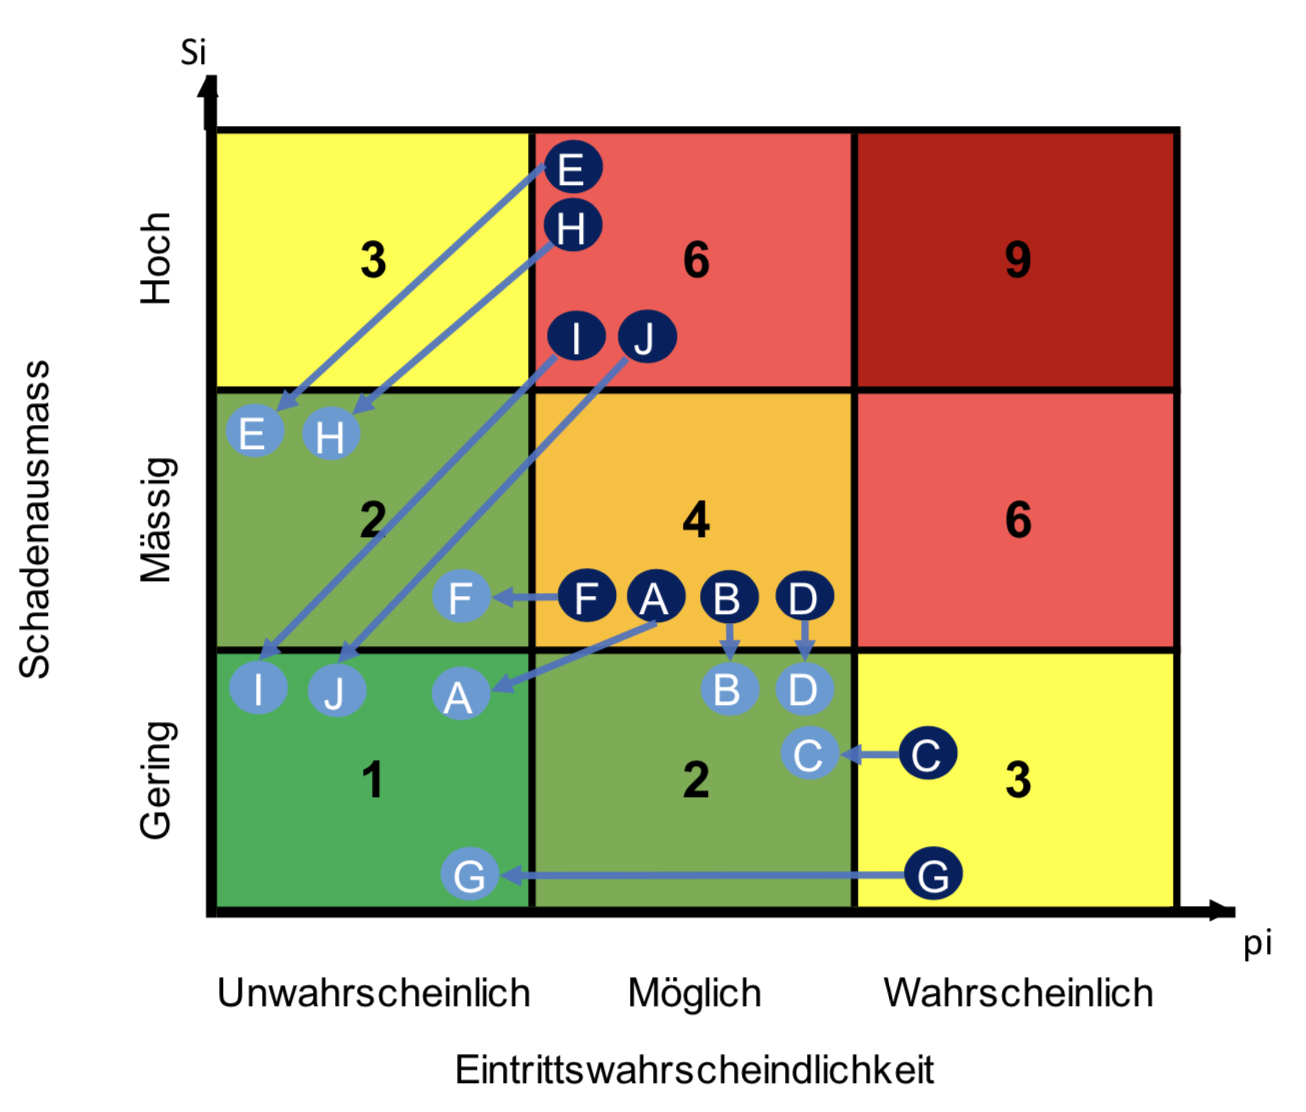
\includegraphics[width=14cm]{Matrix_verschiebung_P2.png}
	\label{fig:Matrix_verschiebung}
\end{figure}


\begin{figure}[H]
	\centering
	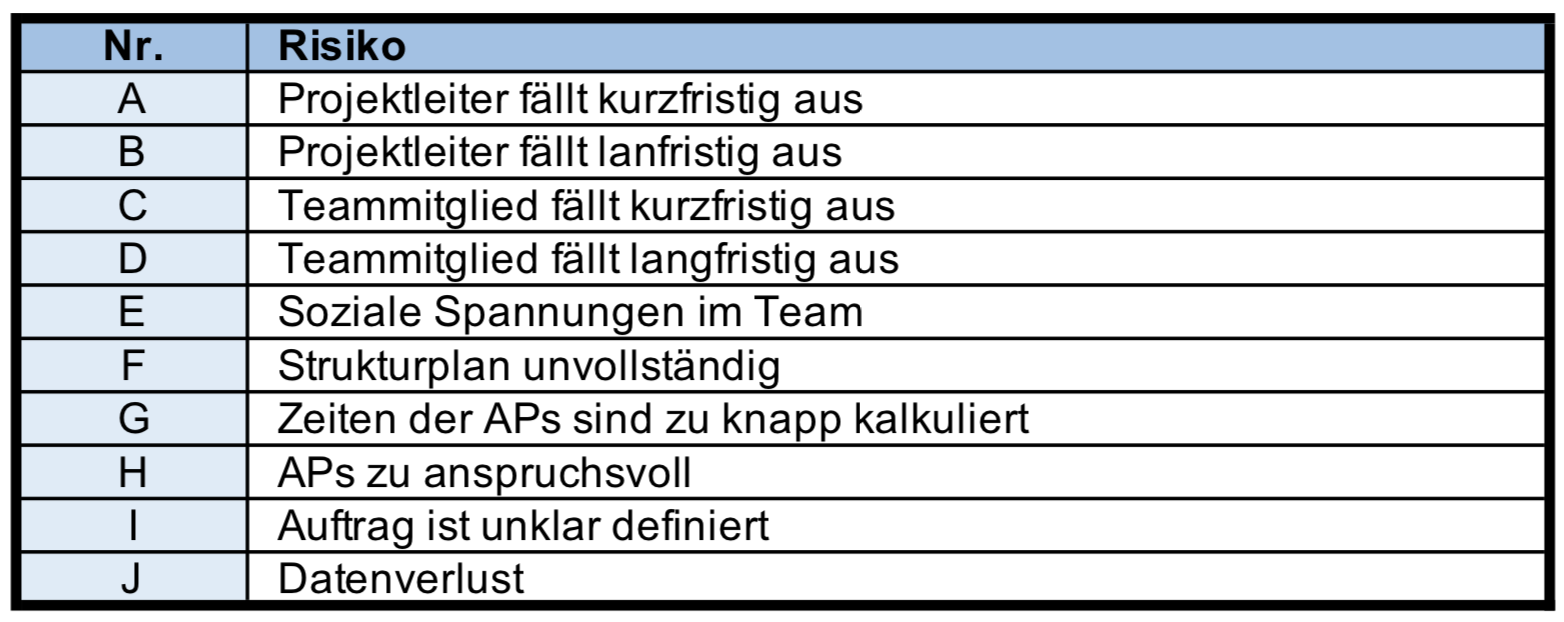
\includegraphics[width=14cm]{Risikouebersicht_P2.png}
	\label{fig:Risikoüebersicht}
\end{figure}

\section{Projektvereinbarung} \label{sec:projektvereinbarung}
\begin{tabular}{l l}
\textbf{Auftraggeber} &\\
&\\
Dr. Luca Dalessandro \\
&\\
&\\
&\\
\rule{6cm}{0.5pt} & \rule{6cm}{0.5pt}\\
Ort, Datum & Unterschrift\\
&\\
&\\
&\\
&\\
&\\
&\\
\textbf{Projektleiter} &\\
&\\
Niklaus Schwegler&\\
&\\
&\\
&\\
\rule{6cm}{0.5pt} & \rule{6cm}{0.5pt}\\
Ort, Datum & Unterschrift\\
\end{tabular}



%%---BIBLIOGRAPHY------------------------------------------------------------------------

{\sloppypar
\selectlanguage{english}	
\setlength{\bibitemsep}{\baselineskip}
\printbibliography[heading=bibintoc]
\label{sec:lit}
}

%%---NOTES for DEBUG---------------------------------------------------------------------
\ifdraft{%Do this only if mode=draft
%%requires \usepackage{todonotes})
\newpage
\listoftodos[\section{Todo-Notes}]
\clearpage
}
{%Do this only if mode=final
}
\end{document}
